% ---------------------------------------------------
% ----- Chapters of the template
% ----- for Bachelor-, Master thesis and class papers
% ---------------------------------------------------
%  Created by C. Müller-Birn on 2012-08-17, CC-BY-SA 3.0.
%  Freie Universität Berlin, Institute of Computer Science, Human Centered Computing. 
%
\chapter{Evaluationen}
\label{chap:evaluation}
		
		Im Rahmen dieser Masterarbeit wurden mehrere Evaluationen durchgeführt, um die
		Genauigkeit der Matcher zu beurteilen. In diesem Prozess wurde etablierte
		Matching Software für ausgewählte Ontologien verwendet, um eine möglichst
		umfangreiche Ergebnismenge für den Vergleich zu haben.
		
		\section{Evaluation 1}
		\label{subsec:Evaluation 1}
		Als erste Evaluation wurde ein Vergleich zwischen einem von Dr. Ing. Alsayed
		Algergawy entwickelten Algorithmus und einem Matching Prozess mit den Simple
		Label und Levenshtein Distance Matchern durchgeführt. Anschließend wurden die
		Ergebnisse händisch begutachtet, um die Qualität der Matchings zu beurteilen. Die
		Algorithmen nehmen als Ausgangsbasis beide die Labels der Elemente der
		Ontologien. Dieser Vergleich dient als Orientierung und erste Überprüfung, ob
		die Matcher anhand von realen Daten grundlegend funktionieren oder schlechte Ergebnisse
		liefern.
		
		\subsection{Verwendete Ontologien}
		Für den Vergleich wurden die Environment Ontology (EnvO) und die Phenotypic
		Quality Ontology (PATO) herangezogen. EnvO wurde entwickelt, um die
		Annotation für jegliche Organismen und biologische Exemplare zu erleichtern.
		Dafür wird ein strukturiertes Vokabular geboten. EnvO besteht aus Wörtern für
		Biome, Umwelteigenschaften und
		Materialien.\footnote{\url{http://www.environmentontology.org/home/about-envo}}
		PATO enthält Begriffe über
		Phänotypen, also das
		Erscheinungsbild von
		Organismen.\footnote{\url{http://obofoundry.org/ontology/pato.html}}
		
		\subsection{Resultat}
		Es wurden 203 gleiche Matchings von beiden Algorithmen gefunden, bis auf neun
		Ergebnisse beschrieben alle das gleiche Konzept, d.h. sie hatten die selbe
		URI.
		Wenn man die Unterschiede in den Ergebnissen betrachtet, also solche, die nur
		einer der beiden Matching Algorithmen gefunden hat, dann hat der Simple
		Ontology Matcher 89 potenzielle Matchings gefunden, während der Algorithmus
		von Dr. Ing. Algergawy 62 vorschlug. Von diesen Matchings war beim Simple
		Ontology Matcher lediglich eines dabei, bei welchem beide Elemente die gleiche
		URI hatten. Bei den Ergebnissen des anderen Algorithmus war dies bei 19
		Matchings der Fall.\\
		Alle Paare und die konkrete Einteilung in die Kategorien sind im Appendix
		\ref{app:first_appendix}
		aufgeführt.
		
		\subsection{Korrektheit der Resultate}
		Die erste Evaluation sollte als erste grobe Einordnung dienen, inwiefern
		der Simple Ontology Matcher seinem Ziel nahe kommt, zwei beliebige Ontologien
		zu vergleichen und Verbindungen zwischen ihnen zu finden. Für die Einordnung
		wurden daher folgende Kategorien verwendet:\\
		\begin{itemize}
		  \item Gleich: Zwei Elemente beschreiben das selbe Konzept.
		  \item Gegenteil: Zwei Elemente sind das Gegenteil voneinander.
		  \item Indirekt: Die beiden Elemente können über ein anderes Elemente.
		  miteinander verbunden werden, unabhängig davon, ob es Teil einer der beiden
		  Ontologien ist.
		  \item Ähnlich: Zwei Elemente sind zwar verbunden, es lässt sich aber keine
		  direkte Verbindung angeben, meist ist eines eine Beschreibung des anderen
		  oder beide haben den selben Wortstamm.
		  \item Keine: Es besteht keine Verbindung und das Matching ist ein false
		  positive.
		  \item Unsicher: Es ist unklar ob zwei Elemente miteinander verbunden sind,
		  da das notwendige Domänenwissen aufgrund von Fachfremdheit fehlt.
		\end{itemize}
		
		Diese Kategorien sind bewusst weit gefasst gewählt. Dadurch ist es
		möglich, eine grobe Übersicht über die Arbeitsweise der Matcher und mögliche
		Arten von Verbindungen zu bekommen und die Ergebnisse einordnen zu können.\\
		Bei der Durchsicht der Ergebnisse fiel schnell auf, dass der Simple Ontology
		Matcher sehr viele Matchings gefunden hat, die zwar verbunden sind, aber keine
		Gleichheit ausdrücken (Kategorien Gegeteil und indirekt).
		Wohingegen der von Dr. Ing. Algergawy verwendete Algorithmus viele Matchings
		gefunden hat, die Gleichheit zwischen den Elementen ausdrücken (Kategorien
		Gleich und Ähnlich).\\
		
		\begin{center}
		\begin{table}[h!]
		\small
		\setlength\tabcolsep{2pt}
		\caption{Kategorisierte Ergebnisse}
		\noindent\makebox[\textwidth]{
			\begin{tabular}{|c|c|c|c|c|c|c|}\hline
			Matching Algorithmus von & Gleich & Gegenteil & Indirekt & Ähnlich & Keine &
			Unsicher \\\hline
			Dr. Ing. Algergawy & 6 (13,95\%) & 0 & 1 (2,32\%) & 16 (37,2\%) & 13
			(30,23\%) & 7 (16,27\%) \\\hline
			Schröter & 1 (1,13 \%) & 40 (45,45\%) & 5 (5,68\%) & 11 (12,5\%) & 21
			(23,86\%) & 10 (11,36\%) \\\hline
			\end{tabular}
		}
		\end{table}
		\end{center}
		Alle Prozentangaben in der Tabelle wurden abgerundet.\\
				
		\begin{figure}[h!]
		\centering
		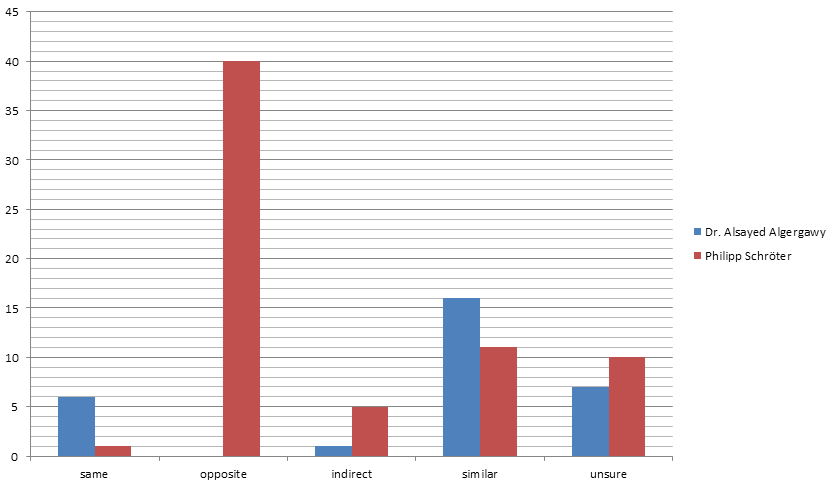
\includegraphics[width=1.0\textwidth]{pics/Vergleich-Algergawy-Schroeter_2016-11-22.png}
		\caption{Vergleich Algergawy Schröter}
		\label{fig16}
		\end{figure}
		
		\subsection{Fazit und Verbesserungen des Simple Ontology Matchers}
		Als erstes wurde für die gleichen Elemente, also solche mit gleicher URI, ein
		eigener Matcher geschrieben und als Bedingung in die anderen Matcher
		aufgenommen, dass die URI nicht mehr gleich sein darf. Dadurch können diese
		trivialen Ergebnisse gezielt in die Ergebnismenge miteinbezogen oder
		ausgeschlossen werden.\\
		Für den Levenshtein Matcher ergibt sich die Verbesserung, dass die obere
		Schranke für mögliche Änderungen nicht nur ein absolutes Maximum benötigt,
		sondern eines, das an die Wortlänge angepasst ist.\\
		Als Gesamterkenntnis hat sich gezeigt, dass es einen Unterschied in der
		Herangehensweise gibt, der zu derartig unterschiedlichen Ergebnissen führt.
		Die übliche Suche nach Verbindungen zwischen Ontologien bezieht sich auf
		Gleichheit oder Ähnlichkeit. Im Rahmen dieser Masterarbeit wurde intuitiv der
		Ansatz gewählt, dass jede möglich Art der Verbindung zu suchen ist, egal
		welcher Art. Ob und wo diese Ansätze sinvoll sind, müssen Experten auf dem
		jeweiligen Gebiet entscheiden, auf dem die Matchings erstellt werden.
		
		\section{Evaluation 2}
		\label{subsec:Evaluation 2}
		Für die zweite Evaluation wurden die zwei Ontologien des \textit{Anatomy track} der
		\textit{2016 Campaign}\footnote{\url{http://oaei.ontologymatching.org/2016/}} der
		\textit{Ontology Alignment Evaluation
		Initiative}\footnote{\url{http://oaei.ontologymatching.org/}} verwendet,
		die \textit{Adult Mouse Anatomy} und ein Teil des \textit{NCI Thesaurus}.\\
		Das NCI Thesaurus beschreibt die menschliche Anatomie, Adult Mouse Anatomy die von
		Mäusen. Ontologien, die aus der Domäne des Anatomy track stammen, sind
		umfangreich, sorgfältig erstellt und beschreiben Konzepte in technischer
		Sprache. Neben ihrer Größe und einer nur zum Teil in natürlicher Sprache
		verfassten Konzeptualisierung unterscheiden sie sich von anderen Ontologien in
		der Verwendung bestimmter Annotationen und Rollen, z.B. häufigen partOf
		Beziehungen. Ein als Referenz vorgegebenes Matching zeigt, dass es eine hohe
		Zahl an eher einfachen Matchings gibt, die mit simplen String Vergleichen gefunden werden
		kann. Gleichzeitig gibt es auch einige Paare, die nicht trivial sind und/oder
		anatomisches Hintergrundwissen benötigen.\cite{OAEI16}\\
		Anhand vorher festgelegter Matcher wurde der im Rahmen dieser Masterarbeit
		entwickelte Simple Ontology Matcher mit dem Referenzergebnis der 2016 Campaign verglichen.
		
		\subsection{Resultat}
		Es wurden Ergebnisse verschiedener Matcher mit der Referenz abgeglichen und
		Precision und Recall berechnet.\\
		
		\subsubsection{Simple Ontology Matcher}
		Da es bei diesem Matcher zwei mögliche Einstellungen gibt, wurden beide
		getrennt getestet. Wenn nur exakt gleiche Labels als Matching ausgewählt
		wurden, fand dieser Matcher 933 Paare. Von diesen waren lediglich 3 nicht in
		der Menge der Referenzergebnisse.\\
		
		Wenn man die zusätzlich gefundenen Ergebnisse pauschal als false positives
		einstuft, ergeben sich folgende Werte (alle Prozentangaben in der Tabelle
		wurden mathematisch gerundet)
		\begin{center}
		\begin{table}[h!]
		\small
		\caption{Vergleich 1 Simple Ontology Matcher OAEI16 Referenz}
		\noindent\makebox[\textwidth]{
			\begin{tabular}{|c|c|c|c|c|}\hline
			Gefunden insgesamt & davon nicht in Referenz & Aus Referenz nicht gefunden &
			Precision & Recall \\\hline
			933 & 3 & 586 & 99,68\% & 62,35\% \\\hline
			\end{tabular}
		}
		\end{table}
		\end{center}
		Wenn man die Ergebnisse nicht nur auf exakte Matchings beschränkt (siehe
		Kapitel \ref{simpleOntologyMatcher}), werden 4373 zusätzliche potenzielle
		Matchings gefunden, also insgesamt 5306. Davon waren 102 zusätzlich auch in der Referenzmenge. Aus diesen Daten ergeben sich
		folgende Werte
		\begin{center}
		\begin{table}[h!]
		\small
		\caption{Vergleich 2 Simple Ontology Matcher OAEI16 Referenz}
		\noindent\makebox[\textwidth]{
			\begin{tabular}{|c|c|c|c|c|}\hline
			Gefunden insgesamt & davon nicht in Referenz & Aus Referenz nicht gefunden &
			Precision & Recall \\\hline
			5306 & 4274 & 484 & 19,46\% & 68,07\% \\\hline
			\end{tabular}
		}
		\end{table}
		\end{center}
		
		Wenn man sich die nicht in der Referenzmenge enthaltenen Ergebnisse ansieht,
		kommt man zu der Erkenntnis, dass der Großteil dieser Ergebnisse trotzdem eine
		korrekte und eindeutige Verbindung haben. Die drei bei der ersten Version des
		Simple Label Matchers gefundenen Paare sind
		\begin{itemize}
		  \item http://human.owl\#NCI\textunderscore C12378
		  (Gastrointestinal\textunderscore System)\\ und
		  http://mouse.owl\#MA\textunderscore 0000323 (gastrointestinal system)
		  \item http://human.owl\#NCI\textunderscore C12685 (Capillary) und\\
		  http://mouse.owl\#MA\textunderscore 0000065 (capillary)
		  \item http://human.owl\#NCI\textunderscore C12919 (Organ\textunderscore
		  System) und\\ http://mouse.owl\#MA\textunderscore 0000003 (organ system)
		\end{itemize}
		Alle drei sind bei näherer Prüfung der Elemente korrekte Matchings. Bei der
		zweiten Version des Simple Label Matchers sind 3943 Paare korrekt erkannte
		Matchings, 41 sind entweder false positives oder eine direkte Verbindung nicht
		sinnvoll. Beispielsweise ist \url{http://human.owl#NCI_C12419 (Head)} und
		\url{http://mouse.owl#MA_0000122} (pancreas head) ein eindeutiger false
		positive. Beim Matching \url{http://human.owl#NCI_C32152}
		(Ascending\textunderscore Frontal\textunderscore Artery) und \url{http://mouse.owl#MA_0000064} (artery)
		ist die Verbindung nicht direkt falsch, aber da es bereits eine Verbindung
		sowohl zwischen \url{http://human.owl#NCI_C32152} (Ascending\textunderscore Frontal\textunderscore Artery)
		und \url{http://mouse.owl#MA_0001960} (frontal artery) als auch zwischen
		\url{http://mouse.owl#MA_0000064} (artery) und
		\url{http://mouse.owl#MA_0001960} (frontal artery) gibt, existiert hier
		bereits eine indirekte Verbindung. Dadurch ist in den meisten Fällen nur
		bedingt sinnvoll, noch eine zusätzliche Verbindung hinzuzufügen. Die
		restlichen 109 Matchings sind ohne entsprechendes Domänenwissen nicht
		eindeutig auf Richtigkeit prüfbar.\\
		Bei Betrachtung der zusätzlichen Matchings und Berechnung nach der Precision
		obiger Formel würden sich folgende Werte für die zusätzlichen Matchings
		ergeben
		\begin{center}
		\begin{table}[h!]
		\small
		\caption{Vergleich 3 Simple Ontology Matcher OAEI16 Referenz}
		\noindent\makebox[\textwidth]{
			\begin{tabular}{|c|c|c|c|c|}\hline
			Gefunden insgesamt & true positives & false positives & nicht verifizierbar & Precision \\\hline
			4274 & 3943 & 222 & 109 & 92,3\% \\\hline
			\end{tabular}
		}
		\end{table}
		\end{center}
		Der Recall ist in diesem Fall nicht ohne weiteres bestimmbar, da hier die
		Richtschnur ein "`perfekter Match"' zwischen den zwei Ontologien wäre.
		Der Transparenz wegen sind die vollständigen Ergebnisse und ihre Zuteilung auf
		\url{insert.link} aufgeführt, aus Platzgründen ist diese Auflistung nicht in
		dieser Arbeit enthalten.\\
		Andere Matcher wurden nicht in diesem Rahmen betrachtet, da erste Tests mit
		ihnen schon vorher keine zufriedenstellenden Ergebnisse mit dem gewählten
		Wörterbuch lieferten.
		Dies ist darauf zurückzuführen, dass das Wörterbuch für die Domäne zu
		allgemein ist und das in diesem Kontext benötigte Vokabular nicht in
		ausreichendem Maße enthalten ist.
		
		\pagebreak[4]